\section{Listas}
\begin{frame}

    \frametitle{Listas}

   \begin{block}{}
     \begin{itemize}
      \item Requisito: conceitos de recursividade e functores dominados!
      \item  Os conceitos são os próximos os das  LPs convencionais
     \item Essencialmente vamos computar sob uma árvore
         binária (cada nó tem duas ramificações)

      \item Lembrando que uma estrutura binária de árvore tem uma
      equivalência com uma árvore n-ária (ver livro de Estrutura de Dados)

       \item Logo,  listas são estruturas flexíveis e poderosas!

    \end{itemize}
    
    \end{block}
    
\end{frame}


\begin{frame}
 % \frametitle{Fluxo do Cálculo Recursivo}
\frametitle{Ilustrando uma Lista em Formato Binário}

\begin{figure}[!htb]
\centering
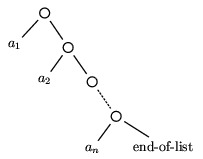
\includegraphics[width=.7\textwidth, height=0.650\textheight]{figures/ilustra-lista-01.jpg}
%\label{fig_ilustra_arv}
\caption{Uma estrutura  Lista -- Homogênea}
\end{figure}

\end{frame}


\begin{frame}
  \frametitle{Ilustrando a Listas}
\begin{figure}[!htb]
\centering
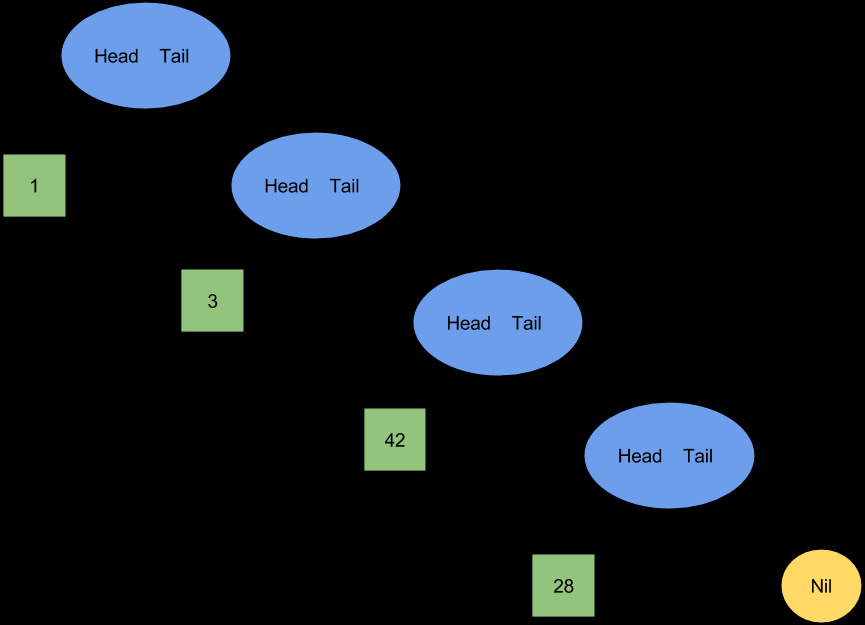
\includegraphics[width=.7\textwidth, height=0.650\textheight]{figures/ilustra-lista-02.jpg}
%\label{fig_arv_recurs_2}
\caption{Listas são inerentemente \textbf{recursivas}!}
\end{figure}
\end{frame}



\begin{frame}
 \frametitle{Exemplificando as Listas}
\begin{figure}[!htb]
\centering
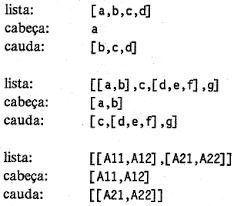
\includegraphics[width=.7\textwidth, height=0.650\textheight]{figures/exemplo_listas_01.jpg}
%\label{fig_arv_recurs_2}
%\caption{Fluxo Recursivo 2}
\end{figure}
\end{frame}

%%%%%%%%%%%%%%%%%%%%%%%%%%%%%%%%%%%%%%%%%%%%%%%%%%%%
\begin{frame}[fragile, allowframebreaks=0.9]
 \frametitle{Sintaxe das Listas}


\begin{block}{Definições iniciais (e recursivas)}
\begin{itemize}


\item Uma lista é uma sequência de objetos;

\item Uma lista é uma estrutura de dados que representa
uma coleção de objetos homogêneos;

\item Uma lista  apresenta uma hierarquia natural, internamente,
em \textit{cabeça} de lista e sub-lista, até o fim da lista.

\end{itemize}
\end{block}
%\lbrack       left bracket [
%\rbrack       right bracket ]

\framebreak
\begin{block}{Notação:}
\begin{itemize}
   \item O símbolo ``\lbrack'' é usado para descrever o início de uma lista,
e ``\rbrack'' para o final da mesma;

   \item Exemplo: seja a lista \lbrack a, b, c, d \rbrack,  logo um predicado cujo
argumento seja algumas letras,  tem-se uma lista do tipo:\\
  \begin{itemize}
  \item letras(\lbrack  a, b, c, d \rbrack )
 \item Onde `a' é  o   \textit{cabeça} (primeiro elemento) da lista
 \item e \lbrack b, c, d \rbrack é uma \textit{sub-lista} que é uma lista!
  \end{itemize}

\item Os elementos de uma lista são lidos da esquerda para direita;

\item  A ``{\em sub-lista}'' \lbrack b,  c, d \rbrack é conhecida como  \textit{resto} ou ``{\em cauda}'' da lista;
        
\item   Esta sub-lista é uma lista, e toda definição segue-se recursivamente.
 \end{itemize} 

\end{block}


\framebreak
\begin{block}{Operador ``{\bf |}'':}

\begin{itemize}
  \item ``{\em  Como vamos distinguir de onde se encontra
a cabeça  da cauda da lista?}'' 

  \item Com as listas novos símbolos foram introduzidos, 
isto é, além dos delimitadores \lbrack \ldots \rbrack, há um 
 novo operador que \textbf{separa} 
 ou \textbf{define} quem é a elemento cabeça da lista e  cauda. 

  \item Este operador é conhecido como
 ``{\em pipe}'' (ou \textit{barra vertical}), simbolizado por ``{\bf |}'', que 
 separa  o lado esquerdo  da direita da lista. 
 
  \item  Esta separação  é necessário para se realizar os 
  \textit{casamentos de padrões} nas linguagens lógicas.

\end{itemize}
\end{block}

\framebreak
\begin{block}{Exemplos de ``{\em casamentos}'':}

% Os exemplos abaixo  ilustram
%como funcionam os casamentos entre variáveis, átomos, etc em listas.
% Atenção em cada exemplo e faça suas próprias conclusões 
%[ de como as listas funcionam.
%\end{itemize}
\begin{small}
\begin{verbatim}
 [ a, b, c, d ] = X
 [ X | b, c, d ]  =  [ a, b, c, d ]
 [ a | b, c, d ]  =  [ a, b, c, d ]
 [ a , b | c, d ]  =  [ a, b, c, d ]
 [ a , b , c | d ]  =  [ a, b, c, d ]
 [ a , b , c , d | [] ]  =  [ a, b, c, d ]
 [] = X
 [ [ a | b , c , d] ] = [ [ a , b , c , d ] ]
 [  a | b , c , [ d ] ] = [  a , b , c , [ d ] ]
 [  _ | b , c , [d ] ] = [  a , b , c , [ d ] ]
 [  a | Y ] = [  a , b , c ,  d ]
 [  a | _ ] = [  a , b , c ,  d ]
 [  a , b | c , d ] = [  X , Y | Z ]
 \end{verbatim}
\end{small}
\end{block}

\framebreak
\begin{block}{Contra-exemplos de ``{\em casamentos}'':}

\begin{verbatim}
 [ a , b | [c, d] ]  !=  [ a, b, c, d ]
 [ [ a , b , c , d] ]  !=  [ a, b, c, d ]
 [  a , b , [ c ] , d, e ]  !=  [ a, b, c, d, e ]
 [ [ [ a ] | b , c , d] ] != [ [ a , b , c , d] ]
 \end{verbatim}

\end{block}

\framebreak
\begin{itemize}
  \item Estes  casamentos de objetos de uma lista
  são também conhecidos  por ``{\em matching}'' 

\item  Devido ao fato de listas modelarem
qualquer estrutura de dados, invariavelmente, seu uso  é extensivo
há  problemas em geral (dos simples a complexos)

\item Porém, alguns cuidados no uso de predicados com backtracking. Acompanhe os
exemplos.

\end{itemize}


\end{frame}


%%%%%%%%%%%%%%%%%%%%%%

\begin{frame}[fragile, allowframebreaks=0.9]
\frametitle{Exemplo: encontrar o comprimento de uma lista}
 
\begin{itemize}
   \item O comprimento de uma lista é o comprimento de sua \textbf{sub-lista}, mais \textbf{um}
   \item O comprimento de uma lista vazia (\lbrack  \rbrack) é zero.
 \end{itemize} 
 
Em Picat, sob uma visão funcional, este enunciado é escrito por:

\begin{verbatim}
comprimento_02( [ ] ) = 0.
comprimento_02([ _ | L ]) = N  => 
             N = 1 + comprimento_02( L ).
\end{verbatim}

\framebreak

Em Picat, sob uma visão lógica, este predicado 
pode ser construído como:

\begin{verbatim}
comprimento_01([],N) ?=> N = 0. 
%%% em PROLOG, apenas comprimento_01([],0). PORQUÊ?
comprimento_01([_|L],N)  => 
             comprimento_01( L , Parcial ), 
             N = 1 + Parcial.
\end{verbatim}

\framebreak
Um ``{\em mapa de memória}'' é dado por:

\begin{center}
\begin{tabular}[c]{|c|c|c|c|c|c|}
\hline
& Regra & X & T & N & N = N+1\\\hline
compto([a,b,c,d],N) & \#2 & a & [b,c,d] & 3 $\rightarrow$ & 3+1$=$4\\\hline
compto([b,c,d],N) & \#2 & b & [c,d] & 2 $\rightarrow$ & $\nwarrow$ 2+1\\\hline
compto([c,d],N) & \#2 & c & [d] & 1 $\rightarrow$ & $\nwarrow$ 1+1\\\hline
compto([d],N) & \#2 & d & [] & 0 $\rightarrow$ & $\nwarrow$ 0+1\\\hline
compto([],N) & \#1 & -- & -- & -- & $\nwarrow$ 0\\\hline
\end{tabular}
\end{center}
 

\end{frame}


\begin{frame}[fragile, allowframebreaks=0.9]
\frametitle{Exemplo: verificar a pertinência de um objeto na lista}

\begin{itemize}
  \item Verifica se um dado objeto pertence há uma  lista
  \item Um método clássico -- muito usado
  \item Tem embutido no Picat: o \textit{menber}
\end{itemize}

Em Picat, sob uma visão funcional, esta função é escrita por:

 \begin{verbatim}
pertence_02( _ , [ ]) = false. 
pertence_02( A, [A|_]) = true. 
% CUIDAR ... em funcoes nao hah ? em ?=> ... 
% sem backtracking em funcoes
pertence_02(A, [B|L]) = X => 
             A != B,
             X = pertence_02(A,L).
\end{verbatim}

%O interessante é observar a versatilidade 
%deste  predicado em várias situações:


\framebreak
Em Picat, sob uma visão lógica, este predicado 
pode ser construído como:
\begin{verbatim}
pertence_01( A, [A|_]) ?=> true. 
% Again, backtracking CONTROLADO ... diferente do Prolog
pertence_01(A,[B|L])  => 
             A != B,
             pertence_01(A,L).
\end{verbatim}

\end{frame}


\begin{frame}[fragile, allowframebreaks=0.9]
\frametitle{Exemplo: adicionar um elemento  em uma lista}

\begin{itemize}
  \item Um objeto é adicionado no início da lista (sem repeti\c{c}ão) caso este já
 esteja contido na lista, a lista original é a retornada:
%  \item 
\end{itemize}

Em Picat, sob uma visão funcional, esta função é escrita por:
 
\begin{verbatim}
add_X_lista_02(X, [ ]) = [X]. 
add_X_lista_02(X, Y) = Z =>
          pertence_02(X, Y) = true,
          Z = Y;
          Z = [ X | Y ].
\end{verbatim}


\framebreak
Em Picat, sob uma visão lógica, este predicado 
pode ser construído como:
\begin{verbatim}

add_X_lista_01(X, [ ], Z )  ?=> Z = [X]. 
add_X_lista_01(X, Y, Z) ?=>
          pertence_01(X, Y),
          Z = Y.
add_X_lista_01(X, Y, Z) =>
          Z = [ X | Y ].

\end{verbatim}

\end{frame}




\begin{frame}[fragile, allowframebreaks=0.9]
\frametitle{Exemplo: união de duas listas}

\begin{itemize}
  \item O método de  união ou concatenação entre duas listas,
 resultando em uma terceira lista

 \item Este predicado é conhecido como \textit{append} ou \textit{concatena}. O \textit{append} está 
pronto na  biblioteca default do Picat

\item Há uma versão simplificada: \texttt{L3 = L1 \textbf{++} L2}

\end{itemize}

Em Picat, sob uma visão funcional, esta função é escrita por:
\begin{verbatim}
uniao_02( [], X ) = X. 
uniao_02( [X|L1], L2 ) = L3 => 
                           L3 = [X | uniao_02( L1, L2 )].
\end{verbatim}

\framebreak

Em Picat, sob uma visão lógica, este predicado 
pode ser construído como:

\begin{verbatim}
uniao_01( [] , X, Y ) ?=> Y = X. 
uniao_01( A , L2, R  ) =>  A = [X|L1] , 
                           R = [X|L3] , 
                           uniao_01( L1, L2, L3 ).
\end{verbatim}

\end{frame}


\begin{frame}[fragile, allowframebreaks=0.9]

\frametitle{Geração de  Listas -- \textit{list comprehension}}

\begin{block}{}
\begin{itemize}
  \item O conceito de \textit{list comprehension} veio da programação funcional
  \item Basicamente serve para criarmos ou gerarmos listas
  \item Bastante útil e pode ser usada em qualquer parte de um código
  
\end{itemize}
\end{block}

\framebreak

Um \textit{list comprehension} tem o seguinte formato
na criação de listas:
\begin{tabbing}
aa \= aaa \= aaa \= aaa \= aaa \= aaa \= aaa \kill
\> \> \texttt{[$T$ : $E_1$ \texttt{in} $D_1$, $Cond_1$, $\ldots$, $E_n$ in $D_n$, $Cond_n$]} 
\end{tabbing}
\begin{itemize}
  \item $T$ é uma termo (uma expressão num caso genérico)
  \item $E_i$ é um padrão de iteração 
  \item $D_i$ é uma expressão de um valor composto, em geral um intervalo de domínio
  \item Opcionalmente,  condições $Cond_1$,$\ldots$,$Cond_n$  são chamados de \textit{termos}
  \item Esta geração de lista tem a seguinte interpretação: \textit{toda tupla de valores $E_1 \in D_1$, $\ldots$, $E_n \in D_n$, 
  se as condições $Cond_i$ forem verdades, então o valor do termo $T$ é adicionado na lista em construção}
\end{itemize}


\framebreak
Um vetor ou matrizes também pode 
ser construídos com um  \textit{array comprehension} e tem
o seguinte formato:
\begin{center}
\texttt{\{$T$ : $E_1$ \texttt{in} $D_1$, $Cond_1$, $\ldots$, $E_n$ in $D_n$, $Cond_n$\}} 
\end{center}

Isto é o mesmo como
%It is the same as:
\begin{center}
\texttt{to\_array([$T$ : $E_1$ \texttt{in} $D_1$, $Cond_1$, $\ldots$, $E_n$ in $D_n$, $Cond_n$])} 

\end{center}
\end{frame}

\begin{frame}[fragile, allowframebreaks=0.9]

\frametitle{Exemplos de \textit{list comprehension}}


\begin{verbatim}
L1 = [I :  I in 1..20]
L2 = [I :  I in 1..20, I>10, I<20]
L3 = [(A,I) : A in [a,b], I in 1..2]
V1 = {I :  I in 1 .. 7}
V2 = {(I,J) :  I in 1 .. 2, J in 11 .. 12}
\end{verbatim}

\end{frame}

%%%%%%%%%%%%%

\begin{frame}[fragile]
\frametitle{Concluindo Listas}

\begin{block}{}
\begin{itemize}
  \item Há muitos predicados e funções prontas sobre listas nos módulos do Picat
  \item Se aprende sobre listas, fazendo muitos métodos
  \item A recursividade em sua modelagem, define a metodologia de se \textit{programar em lógica}
  \item Exercitar-se
  \item Usar as listas em problemas complexos, como na aula de aplicações de buscas.
  
\end{itemize}

\end{block}

\end{frame}





